\chapter{Introduction}
\pagenumbering{arabic}

A concurrent program is any program consisting of multiple interacting tasks,
implemented as separate ``threads of control''.  We will see various patterns
for how the different tasks work together.  For example, the different tasks
might be performing different operations, as part of a pipeline; or they might
be performing the same operation, but on different parts of the data.

The tasks might all execute on the same processor, sharing processor time.  Or
they might operate on several close-coupled processors, within a single
computer.  Or they might be distributed across a network.

The key concern in each case is coordinating the different tasks, to ensure
correct sequencing of interactions or communications between them.

%%%%%%\heading{Processes and threads}

Concurrent tasks can be implemented as either \emph{processes} or
\emph{threads}.

A thread is a single sequentially executing program.  At each point, it is at
a particular place in the program, and has its own \emph{thread-local}
variables and a control stack.  However, different threads may share memory,
and so communicate with one another via shared variables.  This provides for a
low communication overhead.  Threads are normally fairly lightweight, so
context switching (where a processor switches from executing one thread to
another) can be cheap.

A process consists of one or more threads sharing an address space.  However,
different processes have separate address spaces. which protects threads from
each other.  Processes communicate with each other, either using
operating-system calls, or by communicating over a network.  This means that
they have relatively high communication overheads.

In this book we will use threads sharing a single address space.  However,
some of our programs use message passing (only), so the threads could be
replaced by processes in distinct address spaces, or even on different
computers.

The word \emph{concurrent} refers to two or more tasks that overlap in time.
However, they might not ever be running at precisely the same instance:
instead, a processor could be switching between them.  By contrast, the word
\emph{parallel} means that the tasks are running at the same time, on
different hardware.  We will not distinguish much between concurrency and
parallelism in this book.  All of our programs could run on a single
processor, time sharing.  However, we really expect them in parallel, on
different processors, so as to give faster performance. 

%%%%%%%%%%%%%%%%%%%%%%%%%%%%%%%%%%%%%%%%%%%%%%%%%%%%%%%%%%%%

\section{Reasons for concurrency}

Why should we write concurrent programs?

The most obvious reason for using concurrency is that running a program on
multiple processors in parallel will often make the program faster.

\framebox{Improve}

Examples:
%
\begin{itemize}
\item
Scientific computations: e.g.~climate modelling, evolution of a galaxy,
effects of new drugs;

\item
Graphics and image processing;

\item
Combinatorial or optimisation problems: e.g.~scheduling problems, game-playing
algorithms.
\end{itemize}

Typical structures for such programs:
%
\begin{itemize}
\item
Data parallel: each thread/process works on part of the data, with all
threads/processes working in the same way;

\item
Task parallel: different threads/processes do different things.
\end{itemize}
%
% (Much more on this later.)

As we will see, using concurrency might not make a program faster.  There is a
danger that the communication and coordination costs outweigh the benefits of
using extra threads.

%%%%%

\heading{Reasons for concurrency: (2) multi-task systems}

Many systems are responsible for a collection of independent (or
semi-independent) tasks, each with its own data.  Such systems are easier to
program using one single thread or process per task, rather than having a
single monolithic thread that is responsible for all the tasks.

For example, consider a controller for a light, that turns the light on and
off periodically.  Using appropriate library code:
%
\begin{scala}
def controller(light: Light, tOn: Int, tOff: Int) = {
  private var tBase = getCurrentTime
  while(true){
    light.on; sleepUntil(tBase+tOn)
    light.off; sleepUntil(tBase+tOn+tOff); tBase = tBase + tOn + tOff
  }
}
\end{scala}

Now suppose you need to control 1000 lights.  
%
\begin{itemize}
\item
How would you do this with a sequential program?

\item
With a concurrent program it is easy: create one thread or process for each
light, and run them concurrently.
\end{itemize}


More examples:
%
\begin{itemize}
\item
Operating systems;

\item
Real-time controllers for factories, power plants, spacecraft, etc;

\item
Programs with GUIs that must respond to user actions;

\item
Simulations;

\item
Multi-character games.
\end{itemize}

In such multi-threaded multi-task systems, multiple threads or processes run
concurrently on the same processor(s), often with more threads/processes than
processors.  The threads/processes take turns to use the processor(s), under
the control of the operating system.

%%%%%

\heading{Reasons for concurrency: (3) distributed computing}

Many applications make use of services provided by computers that are
physically distributed; these are necessarily concurrent.

Examples:
%
\begin{itemize}
\item 
The Web;

\item
File servers in a network;

\item
Database systems.
\end{itemize}

These applications often use a client-server architecture.

The components might themselves be multi-threaded.

Somewhat similarly, fault-tolerant systems may use redundant components.


%%%%%%%%%%%%%%%%%%%%%%%%%%%%%%%%%%%%%%%%%%%%%%%%%%%%%%%%%%%%

\section{Concurrent architectures}

We will briefly discuss a few different concurrent architectures, to provide
background for the rest of the course.

%%%%%

\heading{Uni-processor multi-threaded systems}

Until early this century, most personal computers had a single processor.
However, they could run multiple (user and operating system) threads.

In such systems, the operating system is responsible for sharing the processor
between threads.  The operating system selects a suitable thread and
executes it until either:
\begin{itemize}
\item
the thread suspends itself, e.g.~waiting for input or output to complete; or

\item
the thread has used up its time allocation, at which point it is interrupted.
\end{itemize}
%
A new thread can then be scheduled.  See an Operating Systems textbook for
more details.

%%%%%

\heading{Thread states}

%\includegraphics[width=12cm]{Pics/threadstates.eps}

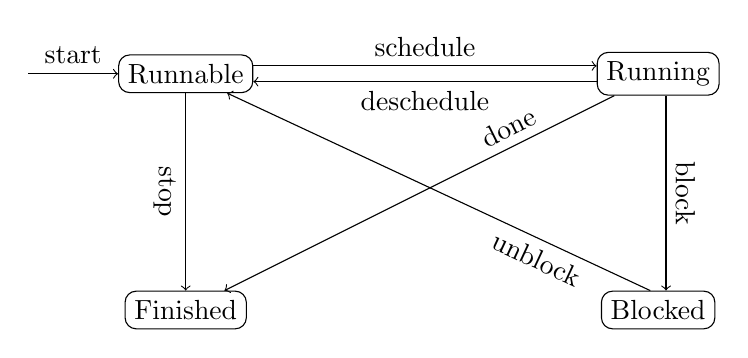
\begin{tikzpicture}
\draw(0,0) node[draw, rounded corners](runnable){Runnable};
\draw[<-] (runnable) -- node[above]{start} (-2,0);
%
\draw(6,0) node[draw, rounded corners](running){Running};
\draw[->] ([yshift = 1mm] runnable.east) -- node[above]{schedule} 
  ([yshift = 1mm] running.west);
\draw[->] ([yshift = -1mm] running.west) -- node[below]{deschedule} 
  ([yshift = -1mm] runnable.east);
%
% \draw (3,3) node[draw, rounded corners](waiting){Waiting};
% \draw[->] (running) -- node[above, sloped]{\scalashape wait} (waiting);
% \draw[->] ([xshift = -1mm] waiting.south) -- node[above, sloped]
%   {\scalashape notify} ([xshift = -1mm] runnable.north);
% \draw[->] ([xshift = 1mm] waiting.south) -- node[below, sloped]
%   {spurious wake-up} ([xshift = 1mm] runnable.north);
%
\draw (0, -3) node[draw, rounded corners](finished){Finished};
\draw[->] (runnable) -- node[below, sloped]{stop} (finished);
\draw[->] (running) -- node[above, sloped, near start]{done} (finished);
%
\draw(6, -3) node[draw, rounded corners](blocked){Blocked};
\draw[->] ([xshift = 1mm] running.south) -- 
  node[above, sloped]{block} ([xshift = 1mm] blocked.north);
\draw[->] ([xshift = -1mm] blocked.north) -- 
  node[below, sloped, near start]{unblock} 
  ([xshift = -1mm] runnable);
%
% \draw(7, 3) node[draw, rounded corners](IOblocked){IO Blocked};
% \draw[->] ([xshift = -1mm] running.north) -- 
%   node[above, sloped]{block for IO} ([xshift = -1mm] IOblocked.south);
% \draw[->] ([xshift = 1mm] IOblocked.south) -- node[below, sloped]{complete IO} 
%   ([xshift = 1mm] running.north);
\end{tikzpicture}

%%%%%

\heading{Shared-memory multiprocessors}

In shared-memory multiprocessors, several processors share one or more
memories.  They are connected by an interconnection network, e.g.\ a memory
bus.  Each processor has its own (fast) cache memory. 

\framebox{Diagram}

%% %
%% \begin{center}
%% \ \includegraphics[width=6cm]{Pics/multiprocessors.eps}\ 
%% \end{center}
% \framebox{Fig 1.2 from Andrews}
% 
The shared memory might be organised hierarchically, particularly in a system
with many processors.

%%%%%

\heading{Cache consistency}

In shared-memory multiprocessor systems, each processor has its own cache.
Values read from the main memory are copied into the cache; a subsequent read
of the same address will read that value from the cache.  If an address is
written to, that write initially happens just in the cache, and later copied
back to the main memory.

Different processors may read and write the same location.  This can be
problematic if the different caches are not consistent.  The specification of
most programming languages include a \emph{memory model} which defines the
degree of consistency that is guaranteed: see later.

%% It is therefore important to keep different caches consistent.  See the
%% Architecture course for details.

%%%%%


\heading{Multi-core processors}

Nowadays, most processors have multiple cores on the same chip.  Each core may
have its own level~1 cache, and they may share a level~2  and level-3 cache.

\framebox{Diagram}

%
%% \begin{center}
%% \includegraphics[height=32mm]{190px-Dual_Core_Generic.svg.ps} \hspace{2cm}
%% (Image from Wikipedia.)
%% \end{center}

Most current off-the-shelf computers are dual-core or quad-core; servers
typically have tens or hundreds of cores.

Multi-core processors provide little speed-up unless the software is designed
to exploit concurrency.

%%%%%

\heading{General-purpose computing on graphics processing units}

A \emph{graphics processing unit} (GPU) is a special-purpose multi-core
processor, originally designed to do graphics processing.  They were designed
to perform many operations in parallel, and so are much faster at floating
point calculations than traditional
CPUs.
%\footnote{\url{http://gpgpu-computing.blogspot.com/}} 

They originally had rather limited functionality.  However, APIs have
been developed that allow them to be used for general-purpose computing.  They
have been used to parallelise many different
applications.
%\footnote{\url{http://en.wikipedia.org/wiki/GPGPU}} 

%%%%%

\heading{Distributed-memory systems}

In distributed-memory systems, each processor has its own private memory.
Processors communicate by message passing, rather than using shared memory. 

\framebox{Diagram}
%
%% \begin{center}
%% \ \includegraphics[width=6cm]{Pics/distributed.eps}\ 
%% \end{center}
% \framebox{Fig 1.3 from Andrews}
%
They might communicate via a high-speed interconnection network, or over a
network, such as a local area Ethernet or the Internet.

%%%%%

%% \begin{slide}
%% \heading{Distributed-memory multicomputers and networks}

%% A \emph{multicomputer} is a distributed-memory system where the processors are
%% physically close, connected by a high-speed interconnection network.

%% In \emph{network systems} (sometimes known as grids), processors
%% communicate over a network, such as a local area Ethernet or the
%% Internet.

%% One can, of course, build distributed-memory systems, where each computer is
%% itself a shared-memory multiprocessor.
%% % multicomputers from shared-memory multiprocessors.
%% \end{slide}

%% %%%%%

%% \begin{slide}
%% \heading{Grid systems and cloud computing}

%% Grid systems are large network systems, often sharing resources across
%% organisations.  They come in two main flavours:
%% %
%% \begin{description}
%% \item[Computational grids,] where computers work together on some
%%   computational task.
%%   % mostly used on problems that require little communication between the
%%   % subtasks. 

%% \item[Data grids,] where there is a huge amount of data to be processed.
%%   % Example types of data include the web (e.g.~web searching), astronomical
%%   % data, data from particle accelerators, genomic sequences.  The data grid may
%%   % be combined with a computational grid that operates on the data.
%% \end{description}


%% Cloud computing can be thought of as ``grids for hire''.  Companies ---such as
%% Amazon, HP, Google, Rackspace--- make grids of computers available to be hired
%% by organisations.  Whether to own your own grid or to hire is mainly an
%% economic decision. 
%% \end{slide}

%%%%%

%% \begin{slide}
%% \heading{Example: Google}

%% Google has 15 data centres worldwide, using about 900,000 servers.
%% %  between 500,000 and several
%% % million processors in total, grouped into clusters of a few thousand
%% % processors.\footnote{{\it Data-Intensive Supercomputing: The case for DISC},
%% %   Randal E. Bryant, CMU-CS-07-128.}
%% Each data centre stores several copies of the web (about 1.2 million terabytes)
%% % (about 200 terabytes),
%% together with indexes to allow efficient searching.  This is continually
%% updated by processes that crawl the web.

%% They use their own custom file system\footnote{{\it The Google File System}, 
%% Sanjay Ghemawat, Howard Gobioff, and Shun-Tak Leung,
%% \url{http://labs.google.com/papers/gfs.html}.}, to distribute the data across
%% servers, providing high performance and fault tolerance. 

%% Each web search uses about 1000 computers, in order to complete the search in
%% about 0.2 seconds.  

%% % Each web search requires about 10 seconds of computer time, but is completed
%% % in about 0.1 seconds by using multiple processors.

%% Their design uses hardware that is low-cost and low-power, rather than fast or
%% reliable. 

%% \vfill
%% \end{slide}

We will mainly consider programs for shared-memory multiprocessors in this
book.

%%%%%%%%%%%%%%%%%%%%%%%%%%%%%%%%%%%%%%%%%%%%%%%%%%%%%%%%%%%%

\section{Disciplined interaction}

The main challenge of concurrent programming is ensuring disciplined
interaction between threads.  Without this, even very simple concurrent
programs can act in unexpected ways.  In particular, it is necessary to ensure
disciplined access to shared variables.

Figure~\ref{fig:race} gives an example that shows what can happen if you allow
undisciplined access to variables.  Such programs are very hard to reason
about.
Appendix~\ref{app:scala} contains a brief introduction to the Scala
programming language.  We will concentrate below on the concurrency aspects of
the program. 

%%%%%

\begin{figure}
\begin{scala}[numbers = left]
import ox.scl._  £\label{line:input}£

/** Program to show the dangers of undisciplined shared variables. */
object Race{
  var x = 0

  /** Thread to increment £x£ 1000 times. */
  def t1 = thread{ for(i <- 0 until 1000) x = x+1 }£\label{line:p}£

  /** Thread to decrement £x£ 1000 times. */
  def t2 = thread{ for(i <- 0 until 1000) x = x-1 }£\label{line:q}£

  /** Parallel composition. */
  def system = t1 || t2£\label{line:system}£

  def main(args: Array[String]) = { run(system); println(x) }£\label{line:main}£
}
\end{scala}% File Race/Race.scala
\caption{A simple program exhibiting a memory race.}
\label{fig:race}
\end{figure}

%%%%%


We use the Scala Concurrency Library (SCL) in this book.  It provides a number
of convenient concurrency primitives.  Line~\ref{line:input} of
Figure~\ref{fig:race} imports this library, so the main primitives can be used
directly; for example, ``|thread|'' is shorthand for ``|ox.scl.thread|''.  (In
later programs, we will tend to omit this |import| statement, for brevity.)

A definition of the form \SCALA{thread\{<code>\}} defines a thread that when
executed will execute \SCALA{<code>}.  For example, line~\ref{line:p} defines
|t1| to be a thread that when executed will increment the shared variable~|x|
1000 times, and line~\ref{line:q} defines |t2| to be a thread that when
executed will decrement |x| 1000 times.  Each thread is of type
|ThreadGroup|\footnote{This type is not the same as the type {\scalashape
    java.lang.ThreadGroup}.}.

If |p| and |q| are |ThreadGroup|s, then \SCALA{p || q} represents their
parallel composition, also of type |ThreadGroup|.  For example,
line~\ref{line:system} defines |system| to be the parallel composition of~|t1|
and~|t2|.  A parallel composition terminates when both components have
terminated.

If |p| is a |ThreadGroup|, then |run(p)| or |p.run| runs~|p|.  Thus the |main|
function at line~\ref{line:main} runs |system|, i.e.~runs |t1| and~|t2| in
parallel, and prints the final value of~|x|.

You might expect that the increments and decrements cancel out, so that the
program always prints~|0|.  In fact, it can give any result between $-1000$
and $+1000$.
%
To understand why, we need to understand how a concurrent program is
executed. 
 
Certain actions can be considered \emph{atomic}; for example a single machine
instruction, or, in the case of a Scala program, a single instruction of the
Java Virtual Machine.  Typical actions include loading a variable into a
register, incrementing or decrementing it, or storing a register into a
variable. 

A sequential program, or a single thread, executes a sequence of atomic
actions.  
%
A concurrent program runs two or more sequential programs: the atomic actions
of the sequential programs are interleaved.

Let's consider a slightly simpler program, where |t1| increments~|x| just
once, and |t2| decrements~|x| just once.  Let's suppose each does this via three
instructions, loading~|x| into a register, incrementing or decrementing it,
and storing the result back in~|x|.  We could write this as
\begin{quote}
\SCALA{LD x; INC; ST x} \qquad and \qquad \SCALA{LD x; DEC; ST x}
\end{quote}
respectively (in fact, the JVM uses slightly longer sequences).

These six instructions can be interleaved in multiple ways.  The table below
considers three interleavings, starting from $\sm x = 0$.
%
\begin{center}
\begin{tabular}{lccccccl}
|x = x+1| & \SCALA{LD x} & \SCALA{INC} & \SCALA{ST x} & \\
|x = x-1| &      &      &     & \SCALA{LD x} & \SCALA{DEC} & \SCALA{ST x}
& ($\sm x = 0$) 
\\
\hline
\SCALA{x = x+1} & \SCALA{LD x} &      & \SCALA{INC} & \SCALA{ST x} & \\
\SCALA{x = x-1} &      & \SCALA{LD x} &     &      & \SCALA{DEC} & \SCALA{ST x}
& (\SCALA{x = -1}) 
\\
\hline
\SCALA{x = x+1} & \SCALA{LD x} &      &     &      & \SCALA{INC} & \SCALA{ST x} & \\
\SCALA{x = x-1} &      & \SCALA{LD x} & \SCALA{DEC} & \SCALA{ST x} &     &
& (\SCALA{x = 1})
\end{tabular}
\end{center}
%
In the first interleaving, all the atomic instructions of the increment are
executed before all the atomic instructions of the decrement, and so we end up
with $\sm x = 0$.  In the second interleaving, both threads read the initial
value of~|x|, then the first thread writes the result of the increment ($1$),
and then the second thread writes the result of the decrement ($-1$),
overwriting the earlier write; hence we end up with $\sm x = -1$.  In the
third interleaving, the writes happen in the opposite order, and so we end up
with $\sm x = 1$.  All other interleavings give one of these three values.  

Returning to the program in Figure~\ref{fig:race}, it should be clear how
different interleavings can produce any result between $-1000$ and~$1000$.

More generally, two actions are \emph{independent} if their order may be
reversed without changing the overall effect.  For example, two actions
concerning distinct variables are independent, as are two reads of the same
variable.  Likewise, the |INC| and |DEC| actions by the above threads affect
only thread-local registers, so are independent of any other actions.
Interleaving of independent atomic actions is not problematic.

However, some actions are non-independent; for example two writes of the same
variable, or a read and a write of the same variable.  Interleaving of
non-independent atomic actions can be problematic.

We say that a program contains a \emph{race} if two non-independent actions
can be interleaved, and one of the interleavings leads to an incorrect
result.  In particular, where those actions are reads or writes of shared
variables, we say that it is a \emph{memory race}.  The program in
Figure~\ref{fig:race} contains memory races, as exhibited by the second and
third interleavings above. 

Different threads can run at different rates: threads can be descheduled and
only later rescheduled; threads may be delayed in memory actions because of
congestion on the memory bus.  It is not feasible to predict which
interleaving will occur.


%%%%% \heading{Caching}

However, there are other reasons why programs with memory races can be
unpredictable.  
%
As described earlier, multiprocessor machines may cache variables.  Caching
can make a program much faster; but it can create problems with concurrent
programs.

When a thread~$t$ first needs the value of a variable~|x|, it will read it
from shared memory, and store a copy in its cache.  If it later needs the
value of~|x|, it may read it from its cache.  However, if some other thread
has updated~|x| in the mean time, thread~$t$ will not see the result of this
update!

Similarly, when a thread~$t$ updates a variable, that update is initially made
only in its cache.  If another thread reads the variable, it will not see the
result of the update.

In the program of Figure~\ref{fig:race}, each thread might read the initial
value of~|x|, perform updates only within its cache, and write the final
value, $1000$ or $-1000$, only at the end.  (However, they are guaranteed to
write their final value when they terminate.)  Thus the final value will be
$1000$ or $-1000$, depending upon which thread writes its value last --- in
fact, on some architectures this seems to happen on most runs of the program.

%%%%% \heading{Compiler optimisations}

Another reason why programs with memory optimisations can be unpredictable
concerns memory optimisations.  The compiler may optimise code, according to
certain rules, to something that is equivalent when run sequentially.
Compiler optimisations are certainly useful, and often produce faster code.
However, the resulting code might not be equivalent when run as part of a
concurrent program.

Consider the code in Figure~\ref{fig:busyWait}.  This uses a variant of the
|thread| function: the construct |thread(name){<code>}| acts like
|thread{<code>}|  but gives the name |name| to the thread; we will see how
this is useful shortly.

In Figure~\ref{fig:busyWait}, it appears that |t1| sets |answer| to |42|, and
then sets |done| to |true|, while |t2| waits for |done| to become true before
reading |answer|: it appears that |t1| is using the variable |done| to signal
to |t2| that it has written to |answer|.

\begin{figure}
\begin{scala}
object BusyWait{
  var answer = 0

  var done = false

  /** Thread to set £answer£ to 42, and then signal to £t2£. */
  def t1 = thread("t1"){ answer = 42; done = true }

  /** Thread to wait for a signal, and read £answer£. */
  def t2 = thread("t2"){
    while(!done){ } // Busy wait.  Don't do this!!!
    val myAnswer = answer; assert(answer == 42)
  }

  /** Parallel composition. */
  def system = t1 || t2

  def main(args: Array[String]) = { 
    for(i <- 0 until 10000){ answer = 0; done = false; run(system); print(".") }
  }
}
\end{scala}
\caption{A program that shows an incorrect signalling technique.}
\label{fig:busyWait}
\end{figure}

However, the code might not act as expected because of compiler
optimisations.  For example, it would be perfectly valid for the compiler to
rewrite the body of~|t1| to
\begin{scala}
  done = true; answer = 42
\end{scala}
%
This is equivalent to the original code as a sequential program, and it a
valid rewrite.  However, the logic around the signal no longer holds.
Likewise, it would be valid to rewrite the body of~|t2| to
\begin{scala}
  val myAnswer = answer; assert(answer == 42)
  while(!done){ } 
\end{scala}
and again the logic around the signal doesn't hold.  Alternatively, it would
be valid for the compiler to rewrite the body of~|t2| to
% 
\begin{scala}
  if(!done){ while(true){ } }
  val myAnswer = answer; assert(answer == 42)
\end{scala}
This is a fairly standard form of rewrite: it avoids rereading the variable
|done|.  Now, this thread can read |done = false| and loop forever, so the
program gets stuck.  In fact, on my machine, the program runs for a few
hundred iterations and then gets stuck: I think the just-in-time compiler
(which optimises Java bytecode to native machine code, while the program is
running) performs an optimisation equivalent to the one above.

When a program does get stuck in this way, typing \texttt{Ctrl}+$\backslash$
(i.e.~holding down the \texttt{Ctrl} key, and pressing the backslash key) in
the terminal produces a thread dump, listing information about all the running
threads, such as giving their current line number in the code.  (This normally
includes several threads that are part of the runtime, rather than the program
in question; these can normally be ignored.)  In particular, this thread dump
uses names given to threads by the |thread(name){...}| construct.  In the
example of the previous paragraph, |t1| is not listed, because it has
terminated; however, |t2| is still at the line corresponding to the |while|
loop.

The style of the loop in~|t2|, where the thread spins, waiting for a condition
to become true, is known as \emph{busy waiting}.  This is normally considered
bad style.  As the above example shows, it often doesn't work!  And even if it
did work, the spinning thread would be consuming computational resources that
might be better used elsewhere.  It would be better for the thread to suspend
until the condition becomes true: we will see in later chapters how to do
this.  

We have seen that programs that contain race conditions are likely to be very
hard to reason about, unpredictable --- and wrong!  However, we want the
behaviour of our programs to be predictable.  We therefore need to design our
programs to avoid race conditions.  In particular, in order to avoid memory
races, we will design our programs so that two threads may not perform
interleaved actions on a shared variable, except if both threads are
performing reads.  We will see that this has the additional benefit of
removing the types of errors introduced by caching or compiler optimisations

%% NSA have issued a report saying that race conditions are the eighth most
%% dangerous programming error.

%%%%%%%%%%%%%%%%%%%%%%%%%%%%%%%%%%%%%%%%%%%%%%%%%%%%%%%%%%%%

\heading{Correctness properties} 

\begin{description}
\item[Safety/correctness:] The results produced by the program are correct.
  Typically this requires that the system state will satisfy an (intended)
  invariant property after every ``action''.

\item[Liveness/progress:] The system as a whole does something useful.
\end{description}

\bigskip

\heading{Performance properties}

\begin{description}
\item[Latency:]
Requests get serviced reasonably quickly.

\item[Throughput:]
The system deals with a high number of requests.
\end{description}

%%%%%%%%%%%%%%%%%%%%%%%%%%%%%%%%%%%%%%%%%%%%%%%%%%%%%%%%%%%%


\section{Summary}

\begin{itemize}
\item
Processes and threads;

\item
Reasons for concurrency;

\item
Concurrent architectures;

\item
Shared variable programs; 

\item
Basics of SCL;

\item
Independent and non-independent actions, race conditions, disciplined
interaction; 

\item
Desirable properties.
\end{itemize}

%%%%%%%%%%%%%%%%%%%%%%%%%%%%%%%%%%%%%%%%%%%%%%%%%%%%%%%

\exercises
%% \section*{Exercises}
%% \markright{Exercises}

\begin{questionS}
Consider a web browser that supports multiple tabs (i.e.~different
tabs for different web pages).  Why might it be beneficial to use
concurrency in the implementation of such a web browser?  Would this
still make sense on a uni-processor computer?  What problems might
arise from such a design?
\end{questionS}

%%%%%

\begin{answerS}
There are two main reasons: ease of implementation, and efficiency.

Building a web browser this way is easier!  The different tabs are largely
independent.  It's far easier to write a thread that deals with a single tab,
and run $n$ such threads, than to write a single thread that deals with all
$n$ tabs.  Each tab thread will probably need to interact with some main
browser thread, but that's relatively straightforward.

In terms of efficiency, concurrency might be used to give better response to
user actions (i.e.\ lower latency), and better overall performance (i.e.\
higher throughput); of these, the former seems more important.

As an example of why a sequential implementation might be unsatisfactory,
consider a user who has two tabs open, one viewing a page that automatically
re-loads every few minutes, and another that the user is actively reading.
Suppose the user tries to scroll down in the second page just after the first
page starts a re-load; then the user has to wait until the re-load completes
before the second page scrolls; this could take several seconds, and so annoy
the user.  (The Firefox browser used to act in this way.)  If the different
tabs used different threads, then they could run concurrently so the user
wouldn't see this delay.  This would still be the case on a uni-processor
machine: the fact that the two processes are competing for the processor would
slow things down a bit, but probably not enough for the user to notice.

The problem is, of course, that two threads might try to access some shared
data (e.g.~the history list) simultaneously, leading to race conditions.
These race conditions can be avoided by careful programming: see the rest of
the book!
\end{answerS}
 % Web browser question. 

\begin{questionS}
\begin{enumerate}
\item
Suppose two threads respectively perform $m$ and $n$ atomic actions
sequentially. How many interleavings of these atomic actions are there?

\item Use your answer to the previous part to give an estimate for the number of
  interleavings of the memory actions from Figure~\ref{fig:race}, where each
  thread performs 2000 memory actions.  \textbf{Hint:} use Stirling's
  approximation, $n! \approx \sqrt{2\pi n} \, (n/e)^n$. 
\end{enumerate}
\end{questionS}

%%%%%%%%%%%%%%%%%%%%%%%%%%%%%%%%%%%%%%%%%%%%%%%%%%%%%%%


\begin{answerS}
\begin{enumerate}
\item There are a total of $m+n$ actions, and the number of interleavings is
  the number of ways of choosing $m$ of those as the actions of the first
  thread.  There is a standard formula for this, namely
  \[\mstyle
  \frac{(m+n)!}{m! \, n!}
  \]
One way to see this is that if we ignore the orderings for each thread, there
are $(m+n)!$ ways of ordering these $m+n$ actions: we can choose the first
action in $m+n$ ways, the second in $m+n-1$ ways, and so on.  However, only a
proportion $1/m!$ of these will respect the order of the first thread, and
only a proportion $1/n!$ will respect the order of the second thread. 


\item
Using the above formula with $m = n = 2000$, and Stirling's approximation, we
get 
\[\mstyle
\frac{4000!}{(2000!)^2}
\approx \frac{\sqrt{2 \pi 4000} \, (4000/e)^{4000}}{
  2 \pi 2000 \, (2000/e)^{4000}}
= \frac{2^{4000}}{\sqrt{2000 \pi}}
\approx 1.7 \times 10^{1202}.
\]
That's a big number!
%% scala> Math.pow(2, 1000)
%% val res1: Double = 1.0715086071862673E301
%% scala> Math.pow(1.0715086071862673,4) /  Math.sqrt(Math.PI * 2000)
%% val res7: Double = 0.016630018093978575
%% So ~ 0.017E1204.
\end{enumerate}
\end{answerS}
 % Count number of interleavings.

\begin{questionS}
\label{exercise:account}
Consider an object representing a bank account, from the following class.
%
\begin{scala}
class Account{
  private var balance = 0

  def credit(value: Int) = atomically{ balance += value }

  def canDebit(value: Int): Boolean = atomically{ balance >= value }

  def debit(value: Int) = atomically{ balance -= value }
}
\end{scala}
%
The ``|atomically|'' pseudocode is intended to indicate that each
procedure is performed atomically (we will see how to do this in a
later chapter).

A thread that wants to perform a debit should first of all call
\SCALA{canDebit}, to avoid the account from going overdrawn; for example
%
\begin{scala}[showstringspaces=false]
  if(account.canDebit(value)) account.debit(value)
  else println("Debit not allowed!")
\end{scala}

What can go wrong if two threads execute the above code at the same
time?  Sketch a solution to this problem.
\end{questionS}

%%%%%

\begin{answerS}
Suppose the current balance is 100, and both threads want to debit 100;
clearly only one should succeed.  Both threads could call
\SCALA{canDebit(value)}, getting back the result \SCALA{true}.  They would
then both call \SCALA{debit}, leading to the account balance becoming $-$100.
This is a \emph{time-of-check to time-of-use} (TOCTTOU) problem: the check
that there is enough money in the account is no longer valid when the debit is
performed.

The point is that the \SCALA{canDebit} action of one thread and the
\SCALA{debit} action of the other are not independent.  This leads to a race
condition.

The obvious way to avoid this problem is to combine the \SCALA{canDebit} and
\SCALA{debit} actions into a single atomic action within the \SCALA{Account}
class.  Something like
%
\begin{scala}
/** Attempt to debit value.  Return true if successful. */
def tryDebit(value: Int): Boolean = atomically{
  if(balance >= value){ balance -= value; true } else false
}
\end{scala}
% 
The calling code (outside the |Account| class) can do the right thing with the
boolean result. 
\end{answerS}

 % Account question.

\begin{questionS}
\label{exercise:stackRace}
Consider the simple implementation of a stack of |Int|s in
Figure~\ref{fig:stackRace}.  This encapsulates a |List[Int]|, holding the
current contents of the stack.  Scala box~\ref{sb:Lists} describes the basics
of the |List| class in Scala. 

%%%%%

\begin{figure}
\begin{scala}
class IntStack{
  private var st = List[Int]()

  /** Push £x£ onto the stack. */
  def push(x: Int) = { st = x :: st }

  /** Pop a value off the stack.  Precondition: the stack is not empty. */
  def pop(): Int = {
    require(!st.isEmpty); val result = st.head; st = st.tail; result
  }

  /** Is the stack empty? */
  def isEmpty: Boolean = st.isEmpty
}
\end{scala}
\caption{A faulty implementation of a stack.}
\label{fig:stackRace}
\end{figure}

%%%%%

\begin{scalaBox}{Lists}
\label{sb:Lists}
The type |List[A]| represents the type of immutable lists containing data of
type~|A|.

A list containing values~|x|, |y| and~|z| can be defined as \SCALA{List[A](x,
  y, z)}; the type parameter~|A| can normally be omitted, as the compiler can
infer it.

If |xs| has type |List[A]|, and |x| has type~|A|, then |x :: xs| is a new
|List[A]| containing~|x| followed by the elements of~|xs|.  The expression
|xs.isEmpty| returns a |Boolean| indicating whether |xs| is empty.  If |xs| is
not empty, then |xs.head| gives its first element, and |xs.tail| gives the
list containing all of~|xs| except the first element.
\end{scalaBox}

%%%%%

The implementation works correctly when used sequentially, but not when it is
used by several threads concurrently.  List as many different things that can
go wrong as possible.  For the purpose of this question, you can ignore errors
caused by caching or compiler optimisations.

You might be wondering what ``correct'' means in this case.  The operations
should appear to take place in a one-at-a-time order, without interfering with
one another, and giving the results one would expect from that order.
Further, the point at which each operation takes place should be at some point
between when the operation is called and when it returns.  That means that if
one operation returns before another is called, they should take place in the
same order; but if two operations overlap in time, they can appear to take
place in either order.

For example, if there are concurrent calls of |push(2)| and |push(3)|,
starting in a state where the stack holds~|xs|, then the final state should
either be |2::3::xs| (the |push(3)| seems to take place before the
|push(2)|), or |3::2::xs| (the |push(2)| seems to take place before the
|push(3)|).  Similarly, if there are concurrent calls to |push(3)| and |pop|,
starting in a state where the stack holds |2::xs|, then either the |pop|
should return~|2| and the final state should be |3::xs| (the |pop| seems to
take place before the |push|), or the |pop| should return~|3| and the final
state should be |2::xs| (the |push| seems to take place before the |pop|).
This property is called \emph{linearization}: we will discuss it in more
detail later in the book.
\end{questionS}

%%%%%%%%%%%%%%%%%%%%%%%%%%%%%%%%%%%%%%%%%%%%%%%%%%%%%%%

\begin{answerS}
The implementation can go wrong in a numbre of ways, described below.  I~will
write ``|pop|-read-1'', ``|pop|-read-2'' and ``|pop|-read-3'' for the three
reads of~|st| within~|pop|.
%
\begin{enumerate}
\item First, the interface of the class does not seem suitable for a stack
  that is used concurrently.  A typical way in which a stack might be used in
  a sequential program is via code such as
\begin{scala}
  if(!stack.isEmpty){ 
    val x = stack.pop(); ... // Do something with £x£.
  }
  else ... // Handle the empty stack.
\end{scala}
However, if this code is used concurrently, the following is possible:
thread~$A$ finds that the stack is not empty; thread~$B$ performs |pop|s to
empty the stack; thread~$A$ attempts a |pop|, and the |require| statement
throws an exception.  Note that this can occur even if each individual
operation call acts atomically.  This is a time-of-check to time-of-use error,
as in the answer to Exercise~\ref{exercise:account}.

It would be better for |pop| to have a signature such as
\begin{scala}
  def pop(): Option[Int]
\end{scala}
either returning a result of the form~|Some(x)|, where |x| is the value
popped, or a result~|None| to indicate that the stack is empty.  (The type
|Option[Int]| contains the union of such values.)  This combines the |isEmpty|
and |pop| operations from the given class.  Client code can treat the result
appropriately in each case.  

\item (This item is somewhat related to the previous.)  Suppose a thread calls
  |pop| when the stack is non-empty, and the subsequent |require| statement
  passes.  However, if another thread then performs |pop|s to make the stack
  empty, |pop|-read-2 will return the empty list, and the expression |st.head|
  will throw an exception.  Alternatively, if the stack becomes empty between
  |pop|-read-2 and |pop|-read-3, then the expression |st.tail| will throw an
  exception.

\item Suppose two threads call |push(2)| and |push(3)| concurrently, and
  suppose both read the same value of~|st|.  Each will write to |st|,
  corresponding to its own operation.  But whichever thread writes first will
  have its value overwritten by the other thread, so the former thread's value
  will be lost.

\item Suppose two threads call |pop| concurrently.  If both read the same
  value of |st| for their |pop|-read-2,  then both will end up
  returning the same value.  Further, it's possible that either one or two
  values are removed from the stack, depending upon the relative orders of the
  reads and writes of |st| within |st = st.tail|.  

\item Now suppose two threads call |push(3)| and |pop|, respectively, and both
  the |push|-read and |pop|-read-2 obtain the same value of~|st|, of the
  form~|2::xs|.  Then the |pop| will return~|2|, but the final value of~|st|
  might be |3::2::xs| (if the |pop|-read-3 and |pop|-write precede the
  |push|-write), or |2::xs| (if the |push|-write precedes the |pop|-read-3 and
  |pop|-write), or |xs| (if~the |pop|-read-3 precedes the |push|-write, which
  precedes the |pop|-write).
\end{enumerate}

However, there is no race concerning the |isEmpty| operation and either a
|push| or a |pop|.  The |isEmpty| will see the result of a |push| if and only
if its read follows the |push|-write, in which case it seems to take place
after the |push|.  Similarly, the |isEmpty| will see the result of a |pop| if
and only if its read follows the |pop|-write, in which case it seems to take
place after the |pop|.
\end{answerS}
 % Stack using List

\begin{question}
\begin{figure}
\begin{scala}
class Queue[A]{
  /** A node in the linked list. */
  private class Node(val datum: A, var next: Node)

  /** The dummy header node. */
  private var head = new Node(null.asInstanceOf[A], null)

  /** The last node in the list. */
  private var last = head

  /** Is the queue empty? */
  def isEmpty = last == head

  /** Add x to the queue. */
  def enqueue(x: A) = {
    val node = new Node(x, null); last.next = node; last = node
  }

  /** Dequeue a value.  Pre: the queue is not empty. */
  def dequeue: A = {
    require(!isEmpty); head = head.next; head.datum
  }
}
\end{scala}
\caption{A sequential queue based on a linked list.}
\label{fig:queue}
\end{figure}

Figure~\ref{fig:queue} gives the implementation of a queue based on a linked
list.  The implementation is correct when the queue is used sequentially.
However, if the queue is used concurrently (i.e.~with two or more threads
calling the operations concurrently), then it can go wrong in a number of
different ways.  

The notion of correctness here is the same as in
Exercise~\ref{exercise:stackRace}.  Operation invocations should appear to
take place in a one-at-a-time order (so without interfering with one another),
giving results as one would expect for a sequential execution.  Further,
invocations should appear to take place in an order compatible with the
temporal order of the invocations; so if one invocation returns before the
other is called, they should have an effect in that order; but if two
invocations overlap in time, they could have an effect in either order.

%% This property is called
%% \emph{linearization}: we'll see it later in the course.  It fits with
%% programmers' mental models.

%
%I have spotted six essentially different ways in which it can go wrong.
Describe how the queue implementation can go wrong when used concurrently, in
as many as possible essentially different ways (I have spotted six essentially
different ways).
%
For the purposes of this question, you should ignore problems caused by
caching or compiler optimisations (those introduce many more ways in which the
implementation can go wrong).
\end{question}

%%%%%%%%%%%%%%%%%%%%%%%%%%%%%%%%%%%%%%%%%%%%%%%%%%%%%%%

\begin{answerI}
%% A thoughtful student might ask ``What does correct mean, here?''  The property
%% we would like is that the operation invocations appear to take place in a
%% one-at-a-time order (so without interfering with one another), in an order
%% compatible with the temporal order of the invocations (so if one invocation
%% returns before the other is called, they should have an effect in that order),
%% and giving results as one would expect for a sequential execution.  This
%% property is called \emph{linearization}: we'll see it later in the course.  It
%% fits with programmers' mental models. 
Here are some problems I spotted.  I'm sure there are others.
%%   In these examples, I will assume that there are no issues concerning
%% caches or compiler optimisations: such issues will introduce many more ways
%% of things going wrong.  %
\begin{enumerate}
\item
The signature isn't really suitable for a concurrent datatype.  Consider code
like the following, to check the precondition of the |dequeue| operation:
%
\begin{scala}
  if(!queue.isEmpty){ val x = queue.dequeue; ... }
\end{scala}
%
A thread~$t$ could check that the queue is non-empty; then other threads could
perform |dequeue|s so as to empty the queue; then when $t$ calls |dequeue|,
the |require| check will fail.  Better would be to have a signature such as
\begin{scala}
  def dequeue: Option[A] = ...
\end{scala}
that returns |None| when the queue is empty, or |Some(x)| if |x| is dequeued.

%%%%%

\item (Somewhat similar to the previous item.)  A thread~$t$ could call
  |dequeue| when the queue is non-empty, so the |require| passes.  But then
  other threads could perform dequeues, to leave the queue empty (so
  \SCALA{head.next = null}).  When $t$ continues, it sets |head| to null, and
  the expression |head.datum| gives a null-pointer exception.

%%%%%

\item Suppose threads~$t_1$ and~$t_2$ call |enqueue| concurrently, enqueueing
  $x_1$ and~$x_2$, respectively.  Each creates a new node, $n_1$ and~$n_2$.
  Then if $t_1$ and~$t_2$ each updates |last.next| to point to their node, in
  that order, the latter will overwrite the former, so $n_1$ isn't connected
  to the list (so the~$x_1$ is lost).  Further, if $t_2$ then updates |last|
  before~$t_1$, then it will end up pointing to~$n_1$, so |last| will no
  longer be reachable from |head|; this means that the results of all
  subsequent enqueues will be lost.

%%%%%

\item Now suppose threads~$t_1$ and~$t_2$ call |dequeue| concurrently, and
  each reads |head| obtaining the same node~$n$.  Then both will set |head| to
  $n$|.next|, and both will return $n$|.datum|: the same value is dequeued
  twice.

%%%%%

\item Suppose thread $t_1$ calls |dequeue|, and advances |head| to node~$n_1$,
  but stalls before reading |head.datum|.  Suppose now thread~$t_2$ calls
  dequeue, advances |head| to $n_2 = n_1$|.next|, and returns $n_2$|.datum|.
  Then thread~$t_1$ can resume, read |head = |$n_2$, and
  return $n_2$|.datum|.  This value has been returned twice, but the value
  in~$n_1$ was lost. 

\item Suppose thread $t_1$ calls |isEmpty| when the list contains two nodes,
  $n_1 = \sm{head}$ and $n_2 = \sm{last}$ with $n_1.\sm{next} = n_2$; and
  suppose it reads $\sm{last} = n_2$ and stalls.  Suppose then thread~$t_2$
  enqueues another value; and then thread~$t_3$ dequeues a value, setting
  $\sm{head} = n_2$.  Then $t_1$ can resume and read $\sm{head} = n_2$; it
  returns |true| even though the queue was non-empty throughout the
  invocation. 
%
  Changing the definition to
  \begin{scala}
  def isEmpty = head == last
  \end{scala}%
  avoids this problem (assuming no compiler optimisations, etc.).
\end{enumerate}

A solution (to the last five issues) is to adapt the implementation so that
each invocation runs in isolation.  This is the approach we'll adopt later in
the course.  
\end{answerI}
 % Queue as linked list



